% **************************************************************************************************************
% A Classic Thesis Style
% An Homage to The Elements of Typographic Style
%
% Copyright (C) 2015 André Miede http://www.miede.de
%
% If you like the style then I would appreciate a postcard. My address 
% can be found in the file ClassicThesis.pdf. A collection of the 
% postcards I received so far is available online at 
% http://postcards.miede.de
%
% License:
% This program is free software; you can redistribute it and/or modify
% it under the terms of the GNU General Public License as published by
% the Free Software Foundation; either version 2 of the License, or
% (at your option) any later version.
%
% This program is distributed in the hope that it will be useful,
% but WITHOUT ANY WARRANTY; without even the implied warranty of
% MERCHANTABILITY or FITNESS FOR A PARTICULAR PURPOSE.  See the
% GNU General Public License for more details.
%
% You should have received a copy of the GNU General Public License
% along with this program; see the file COPYING.  If not, write to
% the Free Software Foundation, Inc., 59 Temple Place - Suite 330,
% Boston, MA 02111-1307, USA.
%
% **************************************************************************************************************
\RequirePackage{fix-cm} % fix some latex issues see: http://texdoc.net/texmf-dist/doc/latex/base/fixltx2e.pdf
\documentclass[ twoside,openright,titlepage,numbers=noenddot,headinclude,%1headlines,% letterpaper a4paper
                footinclude=true,cleardoublepage=empty,abstractoff, % <--- obsolete, remove (todo)
                BCOR=5mm,paper=a4,fontsize=11pt,%11pt,a4paper,%
                ngerman,american,%
                ]{scrreprt}

% ****************************************************************************************************
% Set the encoding of your files. UTF-8 is the only sensible encoding nowadays. If you can't read
% äöüßáéçèê∂åëæƒÏ€ then change the encoding setting in your editor, not the line below. If your editor
% does not support utf8 use another editor!
% ****************************************************************************************************
\PassOptionsToPackage{utf8}{inputenc}
	\usepackage{inputenc}
	
\usepackage{etoolbox}

% ****************************************************************************************************
% Insert the information about your thesis here
% ****************************************************************************************************
\newcommand{\myTitle}{AnSiAn - Android Signal Analyzer\xspace}
\newcommand{\myDegree}{SEEMOO Secure Networking Lab\xspace}
\newcommand{\myName}{Dennis Mantz and Max Engelhardt\xspace}
\newcommand{\myProf}{Prof. Dr.-Ing. Matthias Hollick\xspace}
\newcommand{\mySupervisor}{Jiska Classen}
\newcommand{\myFaculty}{Department of Computer Science\xspace}
\newcommand{\myDepartment}{Secure Mobile Networking Lab\xspace}
\newcommand{\myUni}{\protect{Technische Universität Darmstadt}\xspace}
\newcommand{\myLocation}{Darmstadt\xspace}
\newcommand{\myTime}{\formatdate{01}{09}{2016}\xspace}
\newcommand{\myVersion}{0.1\xspace}

% Choose if you want the standard template with enough space for margin notes or the tempate with small margins
\newtoggle{adrianstyle}
%\toggletrue{adrianstyle} % uncomment this line to have smaller margins
\togglefalse{adrianstyle} % uncomment this line for the standard seemoo template

%********************************************************************
% Note: Make all your adjustments in here
%*******************************************************
\input{classicthesis-config}
\usepackage{tikz}
\usetikzlibrary{dsp,chains}
\usepackage{pgfplots}
%\pgfplotsset{compat=newest}
\usetikzlibrary{positioning}
\DeclareMathAlphabet{\mathpzc}{OT1}{pzc}{m}{it}
\newcommand{\z}{\mathpzc{z}}
\usepackage{float}
\usepackage{scalefnt}

\usepackage{lipsum}

% To cache tikz pictures you have to run pdflatex with -shell-escape or --enable-write18
\ifnum\pdfshellescape=1
\usepgfplotslibrary{external}
\tikzexternalize[prefix=gfxcompiled/]
%\tikzset{external/remake next}
%\tikzset{external/force remake}
\newcommand{\tikzremakenext}{\tikzset{external/remake next}}
%\tikzexternalize[shell escape=-enable-write18]
\else
\newcommand{\tikzremakenext}{}
\fi

%lengths for matlab2tikz
\newlength\figureheight
\newlength\figurewidth 


\usepackage{textpos}
\usepackage{datetime}
\usepackage{changepage}

\usepackage{siunitx}


%********************************************************************
% Bibliographies
%*******************************************************
\addbibresource{Bibliography.bib}

%********************************************************************
% Hyphenation
%*******************************************************
%\hyphenation{put special hyphenation here}
\input{hyphenation}

% hacks and workarounds
\lstdefinelanguage{none}{
  keywords={},
}

% ********************************************************************
% GO!GO!GO! MOVE IT!
%*******************************************************
\begin{document}
\frenchspacing
\raggedbottom
\selectlanguage{american} % american ngerman
%\renewcommand*{\bibname}{new name}
%\setbibpreamble{}
\pagenumbering{roman}
\pagestyle{plain}
%********************************************************************
% Frontmatter
%*******************************************************
\include{FrontBackmatter/Titlepage}
\include{FrontBackmatter/Titleback}
\cleardoublepage%*******************************************************
% Abstract
%*******************************************************
%\renewcommand{\abstractname}{Abstract}
\pdfbookmark[1]{Abstract}{Abstract}
\begingroup
\let\clearpage\relax
\let\cleardoublepage\relax
\let\cleardoublepage\relax

\chapter*{Abstract}

SDR platforms like the \emph{HackRF} enable their users to explore the electromagnetic spectrum. While a wide range of SDR software toolkits, such as gqrx and SDR\#{}, is available for computers, little such software exists for more mobile devices like smartphones and tablets. AnSiAn is a portable open-source SDR toolkit for Android devices that enables users to inconspicuously monitor the wireless spectrum anywhere. In this lab, AnSiAn's performance was improved and its feature set was extended by adding support for the SDRPlay and rad1o SDR platforms, demodulators for RDS and PSK31 and transmission capability for raw I/Q-Files, Morse and PSK31.



\vfill

%\selectlanguage{ngerman}
%\pdfbookmark[1]{Zusammenfassung}{Zusammenfassung}
%\chapter*{Zusammenfassung}
%\lipsum[2]

\selectlanguage{american}

\endgroup			

\vfill
\pagestyle{scrheadings}
\cleardoublepage%*******************************************************
% Table of Contents
%*******************************************************
%\phantomsection
\refstepcounter{dummy}
\pdfbookmark[1]{\contentsname}{tableofcontents}
\setcounter{tocdepth}{2} % <-- 2 includes up to subsections in the ToC
\setcounter{secnumdepth}{3} % <-- 3 numbers up to subsubsections
\manualmark
\markboth{\spacedlowsmallcaps{\contentsname}}{\spacedlowsmallcaps{\contentsname}}
%\begin{adjustwidth}[]{}{-4cm}
\tableofcontents 
%\end{adjustwidth}
\automark[section]{chapter}
\renewcommand{\chaptermark}[1]{\markboth{\spacedlowsmallcaps{#1}}{\spacedlowsmallcaps{#1}}}
\renewcommand{\sectionmark}[1]{\markright{\thesection\enspace\spacedlowsmallcaps{#1}}}
%*******************************************************
% List of Figures and of the Tables
%*******************************************************
\clearpage

\begingroup 
    \let\clearpage\relax
    \let\cleardoublepage\relax
    \let\cleardoublepage\relax
    
    %*******************************************************
    % List of Figures
    %*******************************************************    
    %\phantomsection 
    \refstepcounter{dummy}
    %\addcontentsline{toc}{chapter}{\listfigurename}
    \pdfbookmark[1]{\listfigurename}{lof}
    \enlargethispage{6em}
    \listoffigures
    \enlargethispage{6em}

%	\newpage

    \vspace{8ex}
    

    %*******************************************************
    % List of Tables
    %*******************************************************
    %\phantomsection 
    \refstepcounter{dummy}
    %\addcontentsline{toc}{chapter}{\listtablename}
    \pdfbookmark[1]{\listtablename}{lot}
    \listoftables
        
    \vspace*{8ex}
%   \newpage
    
    %*******************************************************
    % List of Listings
    %*******************************************************      
	  %\phantomsection 
    \refstepcounter{dummy}
    %\addcontentsline{toc}{chapter}{\lstlistlistingname}
    \pdfbookmark[1]{\lstlistlistingname}{lol}
    \lstlistoflistings 

    \vspace*{8ex}
    \newpage
       
    %*******************************************************
    % Acronyms
    %*******************************************************
    %\phantomsection 
    \refstepcounter{dummy}
    \pdfbookmark[1]{Acronyms}{acronyms}
    \markboth{\spacedlowsmallcaps{Acronyms}}{\spacedlowsmallcaps{Acronyms}}
    \chapter*{Acronyms}
    %\glsaddall
    \printglossary[type=\acronymtype,style=long]

\endgroup

\cleardoublepage
%********************************************************************
% Mainmatter
%*******************************************************
\pagenumbering{arabic}
%\setcounter{page}{90}
% use \cleardoublepage here to avoid problems with pdfbookmark
\cleardoublepage


%\part{Project Report}
%************************************************
\chapter{Introduction}\label{ch:introduction}
%************************************************
\glsresetall % Resets all acronyms to not used
\setcounter{table}{0} % fix table numbering

\ac{AnSiAn} is an Android application developed by the Secure Mobile Network Lab (SEEMOO) at 
Technische Universität Darmstadt. It allows for common \ac{SDR} platforms, such as the \emph{HackRF} and the RTL-SDR, to be used with Android devices. This enables a user to inconspicuously sniff and analyze wireless signals on the go.

The project is based on the open-source app RF Analyzer by Dennis Mantz \cite{RFAnalyzer_GitHub}, which features visual browsing through the frequency domain and demodulation of e.g. \ac{AM} and \ac{FM} signals. It has been further developed in 2015 by Markus Grau and Steffen Kreis into what is now \ac{AnSiAn}.

To date, \ac{AnSiAn} adds to following features on top of RF Analyzer:

\begin{itemize}
	\item Waveform graph of received signals
	\item Morse Demodulation and Decoding
	\item RF Scanner that allows for visually scanning a broad spectrum for signals
	\item Restructured \ac{GUI} with better usability
	\item Restructured codebase that follows the \ac{MVC} pattern
\end{itemize}

While this makes \ac{AnSiAn} a powerful tool for mobile signal analysis and processing, further features such as support for additional modulation techniques are desirable. This lab aims to further develop \ac{AnSiAn} in order to extend its feature set, improve app stability and refine existing features.

A detailed description  and explanation of the project goals and their planned schedule is given in \autoref{ch:project_definition}. \autoref{ch:project_progress} covers the actual project progress over time as well as encountered problems, delays and unplanned features in each phase of the project. Details on the design and implementation of features and bugfixes are given in \autoref{ch:design_and_implementation}.
%\autoref{ch:perspective} discusses the future perspective of AnSiAn and suggests what could be done next to further improve the app.
\autoref{ch:conclusion} concludes this documentation.

\chapter{Project Definition\label{ch:project_definition}}

This section defines the features that will be implemented throughout the
project and schedules them into three sprints.

\section{Features}

The new features can be divided into mandatory features, that will have high
priority within this project, and optional features, that will be implemented
if time permits. As can be seen in \autoref{sec:time_schedule}, the third
sprint is reserved for either optional features or completing mandatory
features and the documentation.

\subsection{Mandatory Features}

The following features are scheduled for implementation during the first and
second sprint:
\begin{itemize}
	\item \ac{RDS} demodulation \\
		If the user selects the existing wide-band \ac{FM} demodulation option,
		the app shall try to detect and demodulate any existing \ac{RDS}
		signal along with the audio demodulation. The extracted information
		shall be displayed on the screen.
	\item \ac{PSK31} demodulation \\
		If the user selects either of the single side band demodulation modes
		(\ac{USB} and \ac{LSB}), he or she shall have the option to enable
		\ac{PSK31} demodulation along with or instead of the audio demodulation.
		The demodulated text string shall appear and scroll through the
		analyzer window.
	\item Extraction of RDS-, Morse- and \ac{PSK31}-data to logfiles \\
		If the user selects to demodulate any digital mode, the demodulated
		text shall be written to a log file specified by the user.
	\item Support for the rad1o badge \\
		The rad1o badge, which is a modified low-cost replica of the HackRF,
		shall be supported as a signal source by \ac{AnSiAn}.
	\item Transmission support for HackRF and rad1o \\
		If \ac{AnSiAn} is used with an \ac{SDR} capable of transmitting signals,
		it shall offer options to send signals in the following ways:
		\begin{itemize}
			\item Replay I/O samples from a file
			\item Generate and send Morse code from text
			\item FM-modulate and send audio from a file
		\end{itemize}
\end{itemize}

\subsection{Optional Features}

The optional features are scheduled in the third and last sprint. However,
they will only be added to the feature set if the last sprint is not needed
in order to compensate for delays on the mandatory features. The optional features are
listed in the order of priority:
\begin{itemize}
	\item Walkie-Talkie Mode \\
		The user shall have the possibility to put \ac{AnSiAn} into a Walkie-
		Talkie mode. In this mode, the application will demodulate an FM channel
		and the user can quickly switch between demodulation and transmission
		of audio recorded from the internal microphone.
	\item Packet Radio demodulation\\
		A new mode \emph{Packet Radio} shall be added to \ac{AnSiAn}. Once selected, it shall allow the user
		to tune to a Packet Radio channel and display information about 
		demodulated packets on the screen. If time permits, it might even
		be possible to implement a transmission feature for Packet Radio.
\end{itemize}


\section{Time Schedule}
\label{sec:time_schedule}

The project will have two developers, Dennis Mantz and Max Engelhardt,
working in three sprints. There are three milestones corresponding to
the sprints, labeled Alpha, Beta and Final Version. They each add an independent
and self-contained set of features to the application:

\begin{itemize}
	\item Software Design (due 12.05.)
	\item Sprint 1: Alpha Version (due 09.06.)
	\begin{itemize}
		\item \ac{RDS} demodulation
		\item \ac{PSK31} demodulation
		\item Extraction of \ac{RDS}-, Morse- and \ac{PSK31}-data to logfiles
	\end{itemize}
	\item Sprint 2: Beta Version (due 21.07.)
	\begin{itemize}
		\item Support for the rad1o badge
		\item Transmission support for HackRF and rad1o
		\begin{itemize}
			\item Replay I/O samples from a file
			\item Generate and send Morse code from text
			\item FM-modulate and send audio from a file
		\end{itemize}
	\end{itemize}
	\item Sprint 3: Final Version (due 25.08.)
	\begin{itemize}
		\item Complete leftovers from previous sprints
		\item Walkie-Talkie Mode (optional)
		\item Packet Radio demodulation (optional)
	\end{itemize}
\end{itemize}
\chapter{Project Progress\label{ch:project_progress}}

The software design for each sprint is done ahead of the respective sprint.
This procedure goes along well with the Agile Manifesto which
encourages the design of a complex system in small incremental parts.


\section{Sprint 1: Alpha Version}


\section{Sprint 2: Beta Version}


\section{Sprint 3: Final Version}
\chapter{Design and Implementation}\label{ch:design_and_implementation}

\section{Optimizations and Bugfixes}


\subsection{Memory Optimizations\label{sec:cleanup.mem}}

\begin{figure}
	\centering
	\includegraphics[width=1\linewidth]{gfx/queue_arch}
	\caption{Signal processing architecture with blocking queues}
	\label{fig:queue_architecture}
\end{figure}

The original RF Analyzer application's architecture is based on
blocking queues that synchronize the various signal processing threads
and efficiently manage memory buffers. Unfortunately, this
architecture was partly dropped by the developers of \ac{AnSiAn} when
changing to a new architecture based on the EventBus library. As a result, memory
allocation management does not work as efficiently with the current version
of \ac{AnSiAn}.

Instead of using cycling buffers for inter-thread-communication, \ac{AnSiAn} uses
EventBus to deliver data. Buffers are always allocated freshly
and discarded after use. This results in a high activity of the
\ac{GC} and therefore in a bad overall performance of the app.

\autoref{lst:before_mem_optimization} shows a logcat output of the
app before any optimizations were applied. The \ac{GC} runs approximately 8 times per second
and the slow performance results in stuttering audio demodulation on
older hardware.

\begin{lstlisting}[label=lst:before_mem_optimization, caption=Logcat output
before memory optimizations, language=none]
05-12 17:55:04.060 D/dalvikvm: GC_FOR_ALLOC freed 4347K, 14% free 54695K/62984K, paused 28ms, total 28ms
05-12 17:55:04.180 D/dalvikvm: GC_FOR_ALLOC freed 4321K, 14% free 54737K/62984K, paused 26ms, total 26ms
05-12 17:55:04.300 D/dalvikvm: GC_FOR_ALLOC freed 4507K, 14% free 54705K/62984K, paused 32ms, total 32ms
05-12 17:55:04.420 D/dalvikvm: GC_FOR_ALLOC freed 4454K, 14% free 54759K/62984K, paused 30ms, total 30ms
\end{lstlisting}

In order to fix this performance issue, the architecture is reverted
to using blocking queues and cycling buffers in places where large memory buffers are passed
between threads. EventBus is still used for delivering information
which is not tied to large buffers. A schema of the new architecture
is depicted in \autoref{fig:queue_architecture}. 

In this architecture, the buffers cycle between the threads. The re-usage
of buffers helps to reduce the memory allocation and garbage collection
overhead to a minimum. \autoref{lst:after_mem_optimization} shows the
logcat output after the architecture changes have been applied. The \ac{GC}
only needs to run every 10 to 20 seconds.


\begin{lstlisting}[label=lst:after_mem_optimization, caption=Logcat output
after memory optimizations, language=none]
05-12 17:27:29.230 D/dalvikvm: GC_FOR_ALLOC freed 3233K, 15% free 19706K/23000K, paused 32ms, total 33ms
05-12 17:27:40.780 D/dalvikvm: GC_FOR_ALLOC freed 3528K, 16% free 20235K/23824K, paused 30ms, total 31ms
05-12 17:28:00.110 D/dalvikvm: GC_FOR_ALLOC freed 4130K, 18% free 20338K/24528K, paused 36ms, total 37ms
05-12 17:28:24.520 D/dalvikvm: GC_FOR_ALLOC freed 4263K, 18% free 20341K/24664K, paused 49ms, total 49ms
\end{lstlisting}


\subsection{Bugfixes}


\section{Demodulators}
\subsection{Design and Structural Changes}
\subsection{Re-Implementation of Morse Demodulator}
\subsection{Radio Data System}

The \ac{RDS} signal is transmitted along with wide band \ac{FM}
radio signals to provide additional information about the
radio station and program.

Demodulation of the \ac{RDS} signal is first done in Octave in order to
evaluate the demodulation algorithm. The octave implementation
also helps by providing reference data of the different stages
of demodulation. 

\subsubsection{RDS modulation scheme}

\ac{RDS} uses \ac{BPSK} with Manchester encoding. The signal is
transmitted with an offset of 57 kHz relative to the center frequency
of the mono audio signal (baseband). The 19 kHz pilot tone of wideband \ac{FM}
can therefore be used to retrieve the \ac{RDS} carrier by multiplying
it with itself 3 times. The complete FM spectrum can be seen in
\autoref{fig:quad_demod_spectrum}.

After the \ac{RDS} baseband signal has been retrieved from the \ac{FM} signal
there are multiple ways of demodulating the \ac{BPSK} modulation. A sophisticated
approach tries to recover the phase synchronised \ac{RDS} carrier from the
signal by using e.g. a form of \ac{PLL} or Costas Loop. The symbols can then
be extracted by multiplying the carrier with the modulated signal and apply
a threshold operation to get bits.

A much simpler approach is to analyze the envelope of the signal and dectect
bits based on known shapes of ones and zeros in the waveform.
\autoref{fig:rds_envelope} shows the envelope and the pattern of symbols
which can be detected.

\begin{figure}
	\centering
	\includegraphics[width=1\linewidth]{gfx/rds/rds_waveform.png}
	\caption[RDS envelope waveform after Frequency demodulation]{RDS envelope waveform after Frequency demodulation \cite{1999:iec62106}}
	\label{fig:rds_envelope}
\end{figure}



\subsubsection{RDS coding scheme}

RDS frames are called groups and each group consists of 4 blocks called
A, B, C and D. One block has a length of 16 bit plus a 10 bit checkword.
Block A always contains the \ac{PI} which identifies the radio station.
The content of the other blocks depends on the group type which is located
in block B (see \autoref{fig:rds_group0A}).

\begin{figure}
	\centering
	\includegraphics[width=1\linewidth]{gfx/rds/group0A.png}
	\caption[Coding scheme of RDS: group 0A]{Coding scheme of RDS: group 0A \cite{1999:iec62106}}
	\label{fig:rds_group0A}
\end{figure}

\begin{table}
	\begin{center}
		\begin{tabular}{ c c l }
		 Group Type & Group Version & Description \\\hline
		 0 & A & Basic tuning and switching information only \\
		 0 & B & Basic tuning and switching information only \\
		 1 & A & Programme Item Number and slow labelling codes\\
		 1 & B & Programme Item Number \\
		 2 & A & RadioText only \\
		 2 & B & RadioText only \\
		 3 & A & Applications Identification for ODA only \\
		 3 & B & Open Data Applications\\
		 4 & A & Clock-time and date only \\
		 4 & B & Open Data Applications\\
		 5 & A & Transparent Data Channels \\
		 5 & B & Transparent Data Channels \\
		 6 & A & In House applications or ODA \\
		 6 & B & In House applications or ODA \\
		 7 & A & Radio Paging or ODA \\
		 7 & B & Open Data Applications\\
		 8 & A & Traffic Message Channel or ODA \\
		 8 & B & Open Data Applications\\
		 9 & A & Emergency Warning System or ODA \\
		 9 & B & Open Data Applications\\
		10 & A & Programme Type Name\\
		10 & B & Open Data Applications\\
		11 & A & Open Data Applications\\
		11 & B & Open Data Applications\\
		12 & A & Open Data Applications\\
		12 & B & Open Data Applications\\
		13 & A & Enhanced Radio Paging or ODA\\
		13 & B & Open Data Applications\\
		14 & A & Enhanced Other Networks information only \\
		14 & B & Enhanced Other Networks information only \\
		15 & A & Defined in RBDS [15] only\\
		15 & B & Fast switching information only \\\hline
		\end{tabular}
		\caption{RDS Group Types}
		\label{tab:rds_groups}
	\end{center}
\end{table}

\autoref{tab:rds_groups} lists all group types and their descriptions.
The \ac{RDS} demodulation in AnSiAn only decodes types 0 and 2 because they contain
the basic information which is also often displayed on the radio
receiver.


\subsubsection{Evaluation in Octave}

Developing a signal processing application on Android has many drawbacks. One
issue is that it is very hard to debug the actuall signal processing components
because of the lack of proper tools to visualize and analyze the data that is
being processed. It is also not possible to do rapid prototyping without
sufficient signal processing libaries available. Therefore the \ac{RDS}
demodulator was first developed in Octave and afterwards ported to Android.

For development and testing it is better to work on recorded samples instead
of live captures. This makes tests reproducable and simplify the development
environment. The file was recorded using the record feature of RF Analyzer. It
can be imported to Octave by using the \emph{read\_cuchar\_binary()} script
provided by the GNU Radio project. After each step the produced output data
can be written back to an \emph{IQ} in order to use it in the Android application.
This way it is possible to develop each component of the demodulation process
separately and the output can be visualized on the developing machine.

The demodulation is done in the following steps:
\begin{enumerate}
	\item Downmixing the radio signal to baseband and filter it (see 
		\autoref{fig:rds_downmixing}).
	\item \ac{FM} demodulation (see \autoref{fig:quad_demod_spectrum}).
	\item Downmixing the \ac{RDS} signal to baseband and filter it
		(see \autoref{fig:rds_extraction} b and c).
	\item Take the absolute value of the signal to get the envelope
		that was shown above (see \autoref{fig:rds_waveform}).
	\item Find the beginning of a symbol by searching for a minimum in
		the waveform. From there find the end of the symbol with the
		same strategy. Now determine whether the symbol is a one or a
		zero according to the value of the minimum found in the middle
		of the sample compared to its peaks.
\end{enumerate}

\begin{figure}
\subfloat[Spectrum of the captured signal]{%
  \includegraphics[clip,width=1\linewidth]{gfx/rds/raw_signal_spectrum.png}%
}

\subfloat[Spectrum after downmixing and filtering]{%
  \includegraphics[clip,width=1\linewidth]{gfx/rds/fm_baseband_filtered_spectrum.png}%
}
\caption{FM Modulated Signal}
\label{fig:rds_downmixing}
\end{figure}


\begin{figure}
\subfloat[Signal spectrum after FM demodulation]{%
  \includegraphics[clip,width=1\linewidth]{gfx/rds/quad_demod_spectrum.png}%
  \label{fig:quad_demod_spectrum}
}

\subfloat[RDS baseband spectrum after downmixing]{%
  \includegraphics[clip,width=1\linewidth]{gfx/rds/rds_baseband_unfiltered_spectrum.png}%
}

\subfloat[RDS baseband spectrum after filtering]{%
  \includegraphics[clip,width=1\linewidth]{gfx/rds/rds_baseband_spectrum.png}%
}
\caption{Extracting the RDS signal from the FM signal}
\label{fig:rds_extraction}
\end{figure}

\begin{figure}
	\centering
	\includegraphics[width=1\linewidth]{gfx/rds/rds_magnitude_waveform.png}
	\caption{RDS waveform after take the absolute values}
	\label{fig:rds_waveform}
\end{figure}

The octave code used to execute the steps mentioned above is shown in the
listing below:

\begin{lstlisting}[label=lst:octave_rds, caption=Octave implementation of the RDS demodulator, language=none]
signal = read_cuchar_binary ("~/Downloads/2016-06-01-20-17-18_rtlsdr_100550000Hz_1000000Sps.iq" );
t = linspace(0, length(signal)/1000000, length(signal))';
carrier = e.^(2*pi*-245000*t*i);
down = carrier .* signal;
fl = fir1(300, 100000/1000000*2);
filtered = filter(fl, 1, down);
demod = quad_demod(filtered, 1);
t2 = linspace(0, length(demod)/1000000, length(demod));
rdscarrier = cos(2*pi*-57000*t2)';
rdsbase = demod(1:length(rdscarrier)) .* rdscarrier ;
frds = fir1(300, 2400/1000000*2);
rdsbase_filtered = filter(frds,1,rdsbase);
downsampled = decimate(rdsbase_filtered, 16).*80;
write_cuchar_binary (downsampled, "~/Downloads/rds_baseband_62500sps.iq");
bits = rds_bpsk_demodulate(downsampled, 62500);
rds_decode(bits)
\end{lstlisting}

The \emph{quad\_demod()} function does the quadrature demodulation
(FM demodulation). The \emph{rds\_bpsk\_demodulate()} function is shown
in the following listing:

\begin{lstlisting}[label=lst:octave_rds_bpsk, caption=Octave implementation of the BPSK demodulation, language=none]
function demod = rds_bpsk_demodulate(signal, fs)
  samples_per_symbol = fs/1187.5
  samples_per_symbol = ceil(samples_per_symbol)
  envelope = abs(signal);
  
  % Find the first minimum
  [minimum, idx1] = min(envelope(1:samples_per_symbol))
  
  bits = [];
  while (idx1 + samples_per_symbol*2 < length(envelope))
    % find end of symbol idx2 (minimum near idx1 + samples_per_symbol)
    from = round(idx1+samples_per_symbol*0.75);
    to   = round(idx1+samples_per_symbol*1.25);
    [minimum, idx2] = min(envelope(from:to));
    idx2 = idx2 + from;
    
    % calc mean of all samples between idx1 and idx2 and calc threshold = mean/2
    m = mean(envelope(idx1:idx2));
    threshold = m/2;
    
    % get minimum sample in the middle between idx1 and idx2 ...
    span = idx2 - idx1;
    from = round((idx1+idx2)*0.5 - 0.25*span);
    to   = round((idx1+idx2)*0.5 + 0.25*span);
    [minimum, idxmiddle] = min(envelope(from:to));
    idxmiddle = idxmiddle + from;
    
    % Check whether we have the correct timing. It might be, that idx2 is
    % actually in the middle of a symbol than at its end.
    if (envelope(idx2) > threshold)
      % In this case we find the minimum between idx1 and idx2 and set it
      % as idx1 for the next round:
      %printf("WARNING: Wrong timing. thres=%f < envelope(idx2=%d)=%f\n",threshold,idx2,envelope(idx2));
      idx1 = idxmiddle;
      continue;
    endif
    
    % ... and check it against the threshold
    s = envelope(idxmiddle);
    if (s > threshold)
      bits = [bits 1];
    else
      bits = [bits 0];
    endif
    
    % idx1 = idx2 and continue with the next symbol..
    idx1 = idx2;
    
  endwhile
  demod = bits;
\end{lstlisting}


\subsubsection{Android Implementation}

For the Android implementation two classes are added to the AnSiAn codebase:
\begin{itemize}
	\item BPSK: This class handles the \ac{BPSK} demodulation and can be
		reused by other demodulators using the \ac{BPSK} modulation scheme
		(e.g. PSK31).
	\item RDS: This class integrates in the existing FM class for frequency
		demodulation. It handles the decoding and processing of \ac{RDS}
		groups. 
\end{itemize}

A screenshot of the application demodulating the \ac{RDS} signal of the
\emph{Antenne Frankfurt} station is shown in \autoref{fig:rds_android_screenshot}.

\begin{figure}
	\centering
	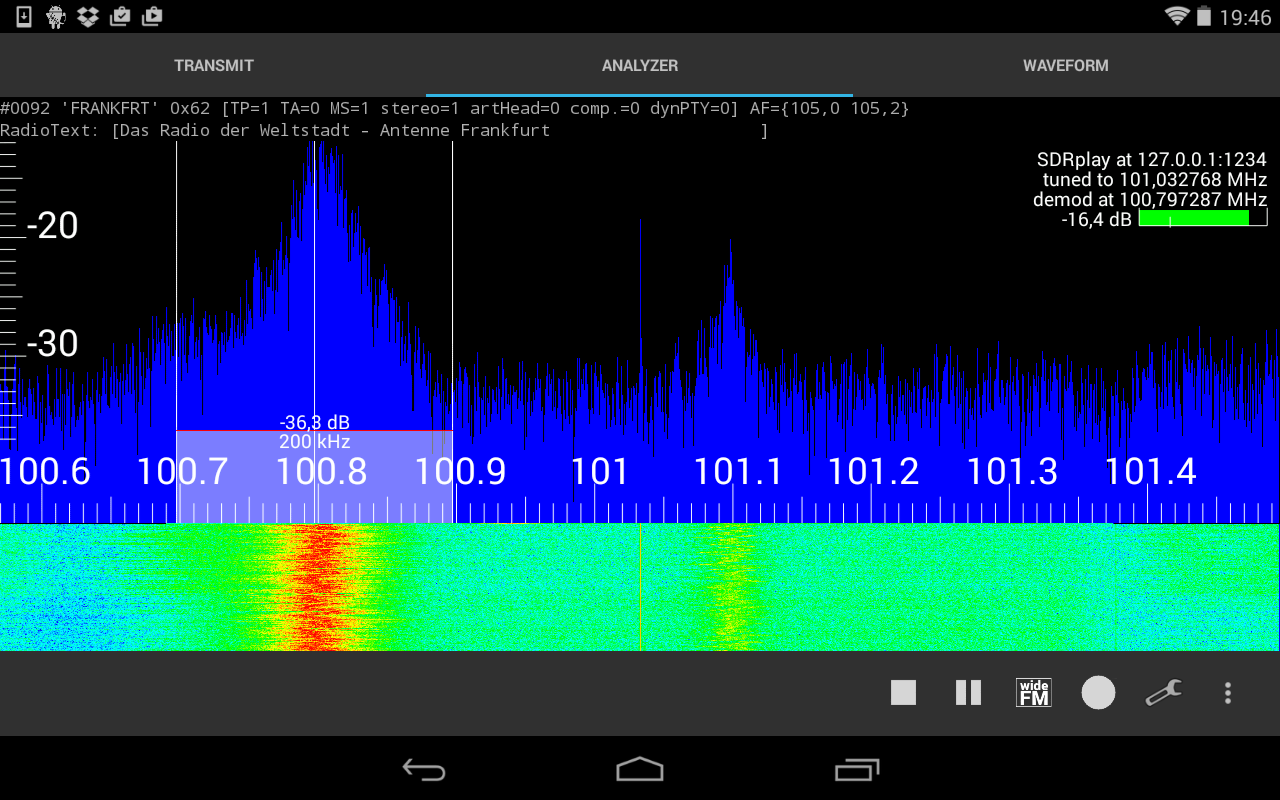
\includegraphics[width=1\linewidth]{gfx/rds/android_screenshot.png}
	\caption{Screenshot of the RDS demodulator on a Nexus 7}
	\label{fig:rds_android_screenshot}
\end{figure}


\subsection{PSK31}


\section{GUI}
\subsection{Reorganization of Preferences}
\subsection{Transmit Tab}

\section{Support for new SDR Platforms}
\subsection{rad1o}
\subsection{SDRPlay}

\section{Transmission}
\subsection{Transmission of Raw I/Q Files}
\subsection{Morse Modulator}
\subsection{PSK31 Modulator}



%\chapter{Perspective\label{ch:perspective}}


\chapter{Conclusion\label{ch:conclusion}}

\ac{AnSiAn} as fork of RF Analyzer has made huge structural changes to the
application architecture in order to implement a clean \ac{MVC} pattern.
Although this has improved the code quality and maintainability it also
introduced issues as described in \autoref{sec:cleanup.mem}. These issues and
their impact on other parts of the app (see \autoref{sec:morse_demod}) had to
be addressed before implementing the new features listed in
\autoref{sec:features}. There were also additional features such as support for
the SDRplay hardware or PSK31 transmission, that were added after the initial
feature list was created and therefore influenced the time schedule.

Nevertheless, all mandatory features apart from some minor exceptions
were successfully implemented. This includes new digital demodulation
modes (PSK31 and RDS), logging of demodulator outputs, support for the
rad1o badge and transmission functionality along with some basic transmission
modes (Morse and PSK31) as well as plain IQ file replay. Not implemented
was the \ac{FM}-modulated transmission of audio files and the optional features:
Walky-Talky-Mode and packet radio demodulation.

Some open tasks and improvements remain to be done in future work on the
application. These include the implementation of the complete transmission
chain as outlined in \autoref{sec:transmission}, additional modulation modes
and improvements on the \ac{BPSK} demodulation algorithm by switching to
a \ac{PLL}-based approach.


%\part{Appendix}
%%********************************************************************
% Appendix
%*******************************************************
% If problems with the headers: get headings in appendix etc. right
%\markboth{\spacedlowsmallcaps{Appendix}}{\spacedlowsmallcaps{Appendix}}
\chapter{Appendix}\label{ch:Appendix}
\glsresetall % Resets all acronyms to not used

\lipsum[8]

% ********************************************************************
% Backmatter
%*******************************************************
\appendix
%\cleardoublepage
%\part{Appendix}
%\include{Parts/Part04}

%********************************************************************
% Other Stuff in the Back
%*******************************************************
\cleardoublepage\include{FrontBackmatter/Bibliography}
\cleardoublepage\include{FrontBackmatter/Declaration}
% ********************************************************************
% Game Over: Restore, Restart, or Quit?
%*******************************************************
\end{document}
% ********************************************************************
